% Options for packages loaded elsewhere
\PassOptionsToPackage{unicode}{hyperref}
\PassOptionsToPackage{hyphens}{url}
%
\documentclass[
  man,floatsintext]{apa6}
\usepackage{amsmath,amssymb}
\usepackage{iftex}
\ifPDFTeX
  \usepackage[T1]{fontenc}
  \usepackage[utf8]{inputenc}
  \usepackage{textcomp} % provide euro and other symbols
\else % if luatex or xetex
  \usepackage{unicode-math} % this also loads fontspec
  \defaultfontfeatures{Scale=MatchLowercase}
  \defaultfontfeatures[\rmfamily]{Ligatures=TeX,Scale=1}
\fi
\usepackage{lmodern}
\ifPDFTeX\else
  % xetex/luatex font selection
\fi
% Use upquote if available, for straight quotes in verbatim environments
\IfFileExists{upquote.sty}{\usepackage{upquote}}{}
\IfFileExists{microtype.sty}{% use microtype if available
  \usepackage[]{microtype}
  \UseMicrotypeSet[protrusion]{basicmath} % disable protrusion for tt fonts
}{}
\makeatletter
\@ifundefined{KOMAClassName}{% if non-KOMA class
  \IfFileExists{parskip.sty}{%
    \usepackage{parskip}
  }{% else
    \setlength{\parindent}{0pt}
    \setlength{\parskip}{6pt plus 2pt minus 1pt}}
}{% if KOMA class
  \KOMAoptions{parskip=half}}
\makeatother
\usepackage{xcolor}
\usepackage{graphicx}
\makeatletter
\def\maxwidth{\ifdim\Gin@nat@width>\linewidth\linewidth\else\Gin@nat@width\fi}
\def\maxheight{\ifdim\Gin@nat@height>\textheight\textheight\else\Gin@nat@height\fi}
\makeatother
% Scale images if necessary, so that they will not overflow the page
% margins by default, and it is still possible to overwrite the defaults
% using explicit options in \includegraphics[width, height, ...]{}
\setkeys{Gin}{width=\maxwidth,height=\maxheight,keepaspectratio}
% Set default figure placement to htbp
\makeatletter
\def\fps@figure{htbp}
\makeatother
\setlength{\emergencystretch}{3em} % prevent overfull lines
\providecommand{\tightlist}{%
  \setlength{\itemsep}{0pt}\setlength{\parskip}{0pt}}
\setcounter{secnumdepth}{-\maxdimen} % remove section numbering
% Make \paragraph and \subparagraph free-standing
\ifx\paragraph\undefined\else
  \let\oldparagraph\paragraph
  \renewcommand{\paragraph}[1]{\oldparagraph{#1}\mbox{}}
\fi
\ifx\subparagraph\undefined\else
  \let\oldsubparagraph\subparagraph
  \renewcommand{\subparagraph}[1]{\oldsubparagraph{#1}\mbox{}}
\fi
\newlength{\cslhangindent}
\setlength{\cslhangindent}{1.5em}
\newlength{\csllabelwidth}
\setlength{\csllabelwidth}{3em}
\newlength{\cslentryspacingunit} % times entry-spacing
\setlength{\cslentryspacingunit}{\parskip}
\newenvironment{CSLReferences}[2] % #1 hanging-ident, #2 entry spacing
 {% don't indent paragraphs
  \setlength{\parindent}{0pt}
  % turn on hanging indent if param 1 is 1
  \ifodd #1
  \let\oldpar\par
  \def\par{\hangindent=\cslhangindent\oldpar}
  \fi
  % set entry spacing
  \setlength{\parskip}{#2\cslentryspacingunit}
 }%
 {}
\usepackage{calc}
\newcommand{\CSLBlock}[1]{#1\hfill\break}
\newcommand{\CSLLeftMargin}[1]{\parbox[t]{\csllabelwidth}{#1}}
\newcommand{\CSLRightInline}[1]{\parbox[t]{\linewidth - \csllabelwidth}{#1}\break}
\newcommand{\CSLIndent}[1]{\hspace{\cslhangindent}#1}
\ifLuaTeX
\usepackage[bidi=basic]{babel}
\else
\usepackage[bidi=default]{babel}
\fi
\babelprovide[main,import]{english}
% get rid of language-specific shorthands (see #6817):
\let\LanguageShortHands\languageshorthands
\def\languageshorthands#1{}
% Manuscript styling
\usepackage{upgreek}
\captionsetup{font=singlespacing,justification=justified}

% Table formatting
\usepackage{longtable}
\usepackage{lscape}
% \usepackage[counterclockwise]{rotating}   % Landscape page setup for large tables
\usepackage{multirow}		% Table styling
\usepackage{tabularx}		% Control Column width
\usepackage[flushleft]{threeparttable}	% Allows for three part tables with a specified notes section
\usepackage{threeparttablex}            % Lets threeparttable work with longtable

% Create new environments so endfloat can handle them
% \newenvironment{ltable}
%   {\begin{landscape}\centering\begin{threeparttable}}
%   {\end{threeparttable}\end{landscape}}
\newenvironment{lltable}{\begin{landscape}\centering\begin{ThreePartTable}}{\end{ThreePartTable}\end{landscape}}

% Enables adjusting longtable caption width to table width
% Solution found at http://golatex.de/longtable-mit-caption-so-breit-wie-die-tabelle-t15767.html
\makeatletter
\newcommand\LastLTentrywidth{1em}
\newlength\longtablewidth
\setlength{\longtablewidth}{1in}
\newcommand{\getlongtablewidth}{\begingroup \ifcsname LT@\roman{LT@tables}\endcsname \global\longtablewidth=0pt \renewcommand{\LT@entry}[2]{\global\advance\longtablewidth by ##2\relax\gdef\LastLTentrywidth{##2}}\@nameuse{LT@\roman{LT@tables}} \fi \endgroup}

% \setlength{\parindent}{0.5in}
% \setlength{\parskip}{0pt plus 0pt minus 0pt}

% Overwrite redefinition of paragraph and subparagraph by the default LaTeX template
% See https://github.com/crsh/papaja/issues/292
\makeatletter
\renewcommand{\paragraph}{\@startsection{paragraph}{4}{\parindent}%
  {0\baselineskip \@plus 0.2ex \@minus 0.2ex}%
  {-1em}%
  {\normalfont\normalsize\bfseries\itshape\typesectitle}}

\renewcommand{\subparagraph}[1]{\@startsection{subparagraph}{5}{1em}%
  {0\baselineskip \@plus 0.2ex \@minus 0.2ex}%
  {-\z@\relax}%
  {\normalfont\normalsize\itshape\hspace{\parindent}{#1}\textit{\addperi}}{\relax}}
\makeatother

\makeatletter
\usepackage{etoolbox}
\patchcmd{\maketitle}
  {\section{\normalfont\normalsize\abstractname}}
  {\section*{\normalfont\normalsize\abstractname}}
  {}{\typeout{Failed to patch abstract.}}
\patchcmd{\maketitle}
  {\section{\protect\normalfont{\@title}}}
  {\section*{\protect\normalfont{\@title}}}
  {}{\typeout{Failed to patch title.}}
\makeatother

\usepackage{xpatch}
\makeatletter
\xapptocmd\appendix
  {\xapptocmd\section
    {\addcontentsline{toc}{section}{\appendixname\ifoneappendix\else~\theappendix\fi\\: #1}}
    {}{\InnerPatchFailed}%
  }
{}{\PatchFailed}
\keywords{big team, science, authorship, credit}
\usepackage{lineno}

\linenumbers
\usepackage{csquotes}
\ifLuaTeX
  \usepackage{selnolig}  % disable illegal ligatures
\fi
\IfFileExists{bookmark.sty}{\usepackage{bookmark}}{\usepackage{hyperref}}
\IfFileExists{xurl.sty}{\usepackage{xurl}}{} % add URL line breaks if available
\urlstyle{same}
\hypersetup{
  pdftitle={Who does big team science?},
  pdfauthor={Erin M. Buchanan1 \& Savannah C. Lewis2},
  pdflang={en-EN},
  pdfkeywords={big team, science, authorship, credit},
  hidelinks,
  pdfcreator={LaTeX via pandoc}}

\title{Who does big team science?}
\author{Erin M. Buchanan\textsuperscript{1} \& Savannah C. Lewis\textsuperscript{2}}
\date{}


\shorttitle{Big Team Science}

\authornote{

Erin M. Buchanan is a Professor of Cognitive Analytics at Harrisburg University of Science and Technology. Savannah C. Lewis is a graduate student at the University of Alabama.

Thank you to Dwayne Lieck for providing an extensive list of large scale projects for this manuscript.

The authors made the following contributions. Erin M. Buchanan: Conceptualization, Data curation, Formal Analysis, Methodology, Project administration, Visualization, Writing -- original draft, Writing -- review \& editing; Savannah C. Lewis: Conceptualization, Data curation, Methodology, Project administration, Writing -- original draft, Writing -- review \& editing.

Correspondence concerning this article should be addressed to Erin M. Buchanan, 326 Market St., Harrisburg, PA 17101. E-mail: \href{mailto:ebuchanan@harrisburgu.edu}{\nolinkurl{ebuchanan@harrisburgu.edu}}

}

\affiliation{\vspace{0.5cm}\textsuperscript{1} Harrisburg University of Science and Technology\\\textsuperscript{2} University of Alabama}

\abstract{%
This paper examined the nature of publications in Big Team Science (BTS): large-scale collaborations between multiple researchers at multiple institutions. These projects can improve research by initiating collaborations that span across the globe, age groups, education levels, and subfields of research. As the number of BTS publications increase, it is useful to explore who is currently involved in BTS projects to determine diversity in both research subject and researcher representation. We examined the diversity of BTS publications and authors across more than half a million articles to investigate where and what is currently published, and author characteristics including differences in career length, publication metrics, affiliation, and affiliation geopolitical regions. Interestingly, BTS publications are increasingly dominated by early career researchers from WEIRD geopolitical regions with Health and Physical Science accounting for the majority of BTS articles. However, the increase in preprints, BTS articles, and non-WEIRD authors across time demonstrate the efforts of the science community to diversify its researchers.
}



\begin{document}
\maketitle

According to the Oxford English dictionary, collaboration is two or more
people working together to achieve a certain goal\textsuperscript{1}.
Collaboration in scientific endeavors involves multiple researchers at
(potentially) multiple institutions to communicate and work together to
advance knowledge in their chosen field. Collaboration can manifest
uniquely in each project dependent on the skill sets, hypotheses, and
perspectives of collaborators. While collaboration is not new in
science, the current interest of ``big team science'' is increasing\textsuperscript{2--4}. Big team science projects
and/or organizations utilize and run on large-scale collaboration to
ensure that diverse populations and ideas are brought into research
projects, which in turn allows for more reliability and generalizability
in the results and method of the study.

BTS appears to be expanding as a result of two sources: 1) increasing
globalization and technology that allows for real-time interdisciplinary
research, and 2) expanding interest in reproducibility, replication, and
generalizability\textsuperscript{5--7}. Technological
advances have provided easier ways to collaborate with people who are
from other universities and countries through document sharing platforms
(e.g., Google, GitHub, and the Open Science Framework), video chatting
platforms (e.g., Zoom, Microsoft Teams), and messaging and project
management platforms (e.g., Slack, Trello, when2meet, etc.). The
credibility movement seems to suggest that by having both collaborations
that span across the globe and subfields of research areas, age groups,
and education levels should help to drive science in the path of better
materials, reliability, generalizability and more robust sample sizes
(when necessary) in a study\textsuperscript{8--10}.

The credibility movement was originally defined by a focus on large
scale replications used in collaborative environments\textsuperscript{11}.
Generally, the movement appears to have been driven by early career
researchers (i.e., those who are within five years of their first
appointment)\textsuperscript{12}; however, there are no large meta-scientific
investigations on this specific topic to date. Potentially, the lack of
investigation is tied to the newness of the large-scale research in many
fields, as it is only in recent years that publications like the Open
Science Collaboration\textsuperscript{13}, Many Labs
Collaborations\textsuperscript{14--20} or the first papers from the
Psychological Science Accelerator\textsuperscript{21--27}. Generally, the researcher incentive for
replication was low for three reasons. First, journals often prioritize
``novel'' or new results which led to rejection of replication manuscripts
and publication bias\textsuperscript{28--30}. Second,
the ``failure'' to replicate was often placed on the replication team as
``bad science'' rather than a careful consideration of publication biases
and (potential) questionable research practices\textsuperscript{5,18}. Last, why should someone want to spend time and resources
on an answer we already ``know''\textsuperscript{31,32}?

However, the success and interest in the large-scale reproducibility
projects\textsuperscript{13,33}, paired
with the meta-scientific publications focusing on researcher practices
and incentive structures\textsuperscript{34,35} led to a
change in journal guidelines and incentives for researchers interested
in participating in large-scale replication studies\textsuperscript{36--39}. For example, the support
for Registered Reports, papers accepted before the data has been
collected\textsuperscript{40,41}, and entire sub-sections of
journals devoted to only replication studies (e.g., \emph{Nature, Royal
Society Open Science, Advances in Methods and Practices in Psychological
Science}) has allowed researchers to invest in projects that they know
should be published when the project is complete. Further, the
implementation of the Transparency and Openness Guidelines\textsuperscript{38}
and the Contributor Role Taxonomy (CRediT) system\textsuperscript{42} have
pushed journals and researchers to promote more open, inclusive
publication practices.

The credibility movement has been mirrored by the calls for
diversification or de-WEIRDing (e.g., Western, Educated, Industrialized,
Rich, and Democratic) scientific research\textsuperscript{43--45} by improving representation in research samples. Like the
large-scale studies in Physics\textsuperscript{46,47} and
Biology\textsuperscript{48}, the Social Sciences struggle to represent the
breadth of humanity across both researcher and population
characteristics. Now, grassroots organizations, such as the
Psychological Science Accelerator\textsuperscript{26}, ManyBabies
(\url{https://manybabies.github.io/}), NutNet (\url{https://nutnet.org/}), and
DRAGNet (\url{https://dragnetglobal.weebly.com/}) can begin to tackle these
issues by recruiting research labs from all over the globe to provide
diversity in geographic, linguistic, and researcher representation.
Publications have examined the global understanding of morality, face
processing, COVID-19 information signaling, and more\textsuperscript{21,23--25,27,49}. While these organizations and one-time groups
for BTS studies have provided an incredible wealth of data for the
scientific community, we do not yet know exactly \emph{who} is involved with,
and benefits from, the BTS and credibility movement. Publications on BTS
generally explore challenges, lessons learned, and the need for BTS\textsuperscript{2,3}.

Therefore, the goal of this manuscript is to examine the \emph{people}
involved in BTS projects. We specifically examined the themes of
inclusivity, research careers, and research globalization. We see an
increasing interest and number of publications in BTS but we do not yet
know if this uptick in large-scale projects has diversified the \emph{people}
involved in BTS. While a few publications have noted that BTS appears to
be early career researchers\textsuperscript{12}, no one has systematically
investigated this perception. Further, it is unclear if the focus of
de-WEIRDing science has only focused on the representation of the
research participants or if it has also improved the representation of
researchers outside of North America and Europe. Last, who runs these
BTS projects? Do we see an increase in diversity for the authors who
generally receive the most credit for these projects (i.e., first
several author(s) and last author)? As hiring and promoting practices
often place a heavy weight on publications and especially ``influential''
publications, it becomes necessary to critically examine the
representation present in authorship in BTS projects.

\hypertarget{research-questions}{%
\section{Research Questions}\label{research-questions}}

\begin{itemize}
\tightlist
\item
  Research Question 1: What publication sources publish big team
  science papers?
\item
  Research Question 2: What are the types of articles that are being
  published in big team science?
\item
  Research Question 3: Who is involved in big team science?
\end{itemize}

This manuscript was preregistered with the same conceptual ideas using
Google Scholar and ORC-ID databases (\url{https://osf.io/f2dtr}) but then
was updated with access to the Scopus database for a broader picture of
BTS projects (\url{https://osf.io/fheun}). All materials and code can be
found on our OSF page: \url{https://osf.io/cgx6u/} or corresponding GitHub
archive: \url{https://github.com/doomlab/big_team_who}.

\hypertarget{method}{%
\section{Method}\label{method}}

\hypertarget{publications}{%
\subsection{Publications}\label{publications}}

We have defined BTS publications as publications with at least ten
authors at ten different institutions that were published in
peer-reviewed journals or had posted a full paper pre-print. We used
data from 1970 and forward in the Scopus database, as it is noted online
that this time period includes cited references for calculation of
several of our variables described below. We will analyze our results
based on four subject areas present in the Scopus database: Physical
Sciences, Health Sciences, Social Sciences, and Life Sciences. We
filtered the database to include articles, articles in press, business
articles, conference papers, data papers, preprints, and surveys using
Elsevier's classification system. This project was supported by access
to the Scopus database through the International Center for the Study of
Research.

\hypertarget{data-curation}{%
\subsection{Data Curation}\label{data-curation}}

\hypertarget{rq1-publisher-information}{%
\subsubsection{RQ1: Publisher Information}\label{rq1-publisher-information}}

We extracted the following information for publication sources: the name
of the publication (source title), subject area (both the large four
subject areas and the smaller four digit all science journal
classification {[}ASJC{]} code), and the journal impact using the Source
Normalized Impact per Paper (SNIP).

\hypertarget{rq2-publication-information}{%
\subsubsection{RQ2: Publication Information}\label{rq2-publication-information}}

For each publication of the identified BTS publications, we examined the
full four digit ASJC subject areas codes for each of the larger four
subject areas and the keywords present for these publications.

\hypertarget{rq3-author-information}{%
\subsubsection{RQ3: Author Information}\label{rq3-author-information}}

The author list was extracted from each publication. Next, we used the
author and affiliation arrays to curate a list of all publications and
author information included in BTS papers to calculate the variables
described below.

\textbf{\emph{Career Length}}. Career length for each author was defined as the
year of the first publication minus the current year listed for each
author.

\textbf{\emph{Institution and Geopolitical Region}}. We used the affiliation ids
and country to gather information about the places of education and/or
employment for authors. Geopolitical region was created by binning these
codes into United Nation Regions.

\textbf{\emph{Education}}. We collected degree information from the author table.
Information on this variable is in the appendix.

\textbf{\emph{Types of Publications}}. We took information from the publication
type variable for each author's publications to present information
about the types of papers BTS authors publish. Information on this
variable is in the appendix.

\textbf{\emph{Publication Metrics}}. For each author, we calculated the total
number of publications, and the h-index. The h-index represents the
highest \emph{h} number of publications that have at least \emph{h} citations.
\emph{h}-count was only used for descriptive statistics.

\hypertarget{results}{%
\section{Results}\label{results}}

We used the 95\% confidence interval to make decisions on predictor or
effect size differences from zero. The confidence interval that does not
include zero would be considered different from zero (to four decimal
places). We made no directional predictions.

\hypertarget{rq1-publisher-information.}{%
\subsection{RQ1: Publisher Information.}\label{rq1-publisher-information.}}

\emph{Number of articles}. The total number of articles included in this
analysis was 510334 including 445301 Health Sciences
articles, 228194 Physical Sciences articles, 26652
Social Sciences articles, and 307514 Life Sciences articles.
Articles could be classified into multiple categories. Figure
\ref{fig:fig-pub-time} shows the number of articles published across
time for each of the four large subject areas.

\begin{figure}
\centering
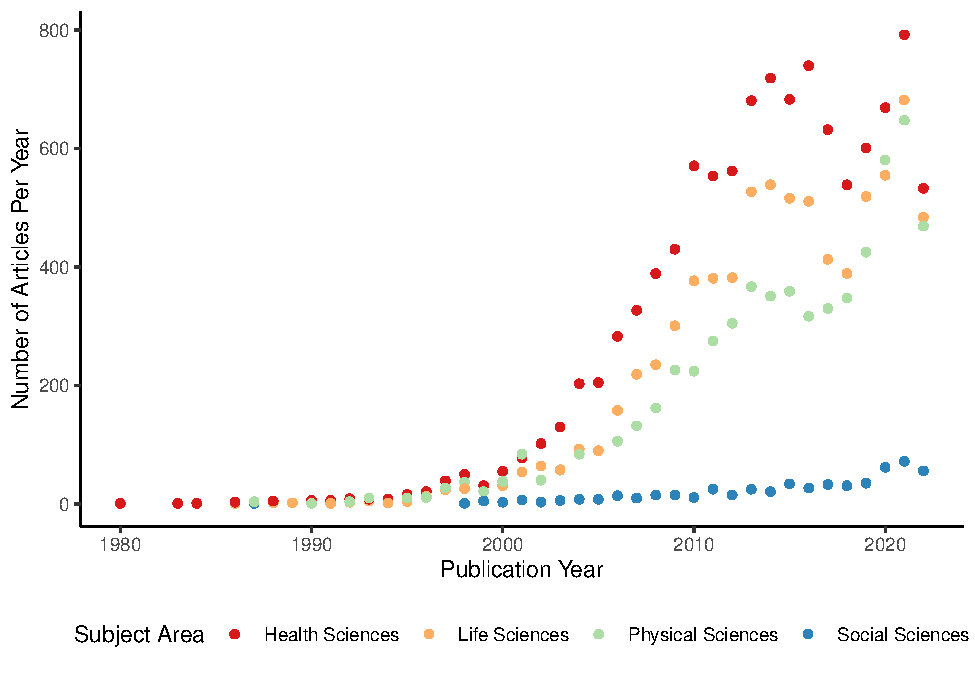
\includegraphics{manuscript_scopus_files/figure-latex/fig-pub-time-1.pdf}
\caption{\label{fig:fig-pub-time}Number of big-team science publications separated by four large subject areas across years. All four subject areas show an exponential number of publications in the last decade.}
\end{figure}

\emph{Number of journals}. The number of distinct journals big team science
articles were published in was 14924 with 6559
journals in Health Sciences, 5787 journals in Physical
Sciences, 2500 journals in Social Sciences, and
4187 journals in Life Sciences. The descriptive statistics
for the Source Normalized Impact per Paper is presented in the
supplemental materials with a comparison for all papers.

\hypertarget{rq2-publication-information.}{%
\subsection{RQ2: Publication Information.}\label{rq2-publication-information.}}

Publication interest area was summarized by the four large subject areas
creating a word cloud plot of the total number of publications within
the ASJCs. Figure \ref{fig:fig-clouds} displays that the Health
Sciences tends to publish within medicine and oncology, with a
corresponding focus of cancer research and genetics for the Life
Sciences. The Physical Sciences was mostly dominated by physics
research, chemistry, and ecology. The BTS publications in the Social
Sciences are mostly within psychology, education, and health.

\begin{figure}
\centering
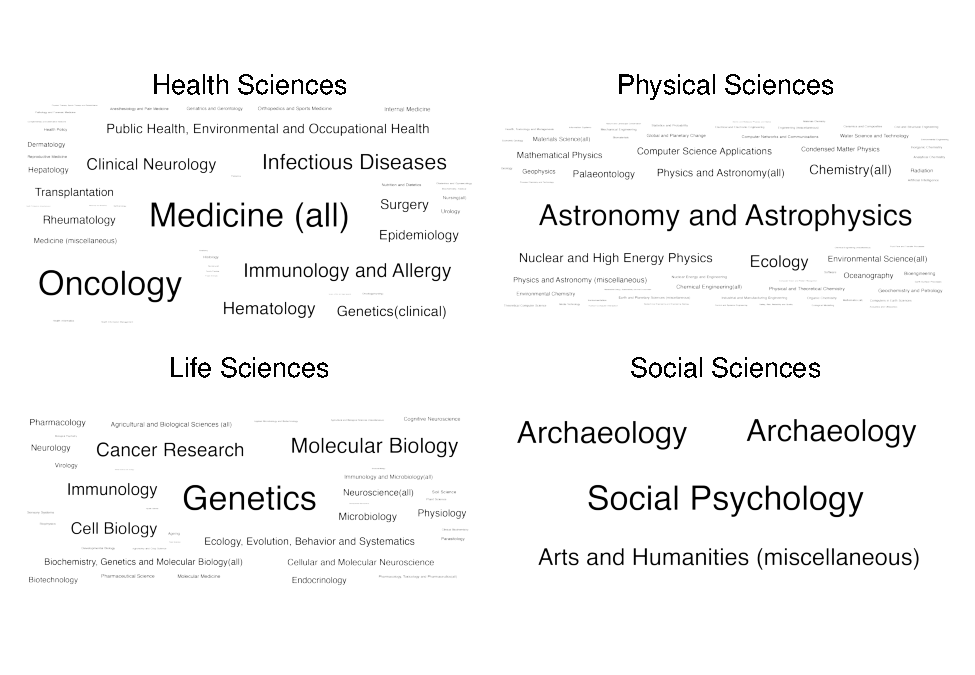
\includegraphics{manuscript_scopus_files/figure-latex/fig-clouds-1.pdf}
\caption{\label{fig:fig-clouds}Journal Areas for Big-Team Science Publications by Subject Area. Larger words indicate more publications in those ASJC areas.}
\end{figure}

\hypertarget{rq3-authors.}{%
\subsection{RQ3: Authors.}\label{rq3-authors.}}

The total number of unique authors across all publications was
3047067. The mean number of authors per publication was \emph{M} =
49.31 (\emph{SD} = 212.98, \emph{Med} = 18) with a
range of 10 to 5568. The median and average
number of authors by subject area are displayed in Figure
\ref{fig:fig-author-year}. In general, the average and median number of
authors increased over time, with the exception of the skew in the
Physical Sciences. Interestingly, the effect in the Physical Sciences
appears to be declining toward the general trends seen in other areas in
the last few decades.

\begin{figure}
\centering
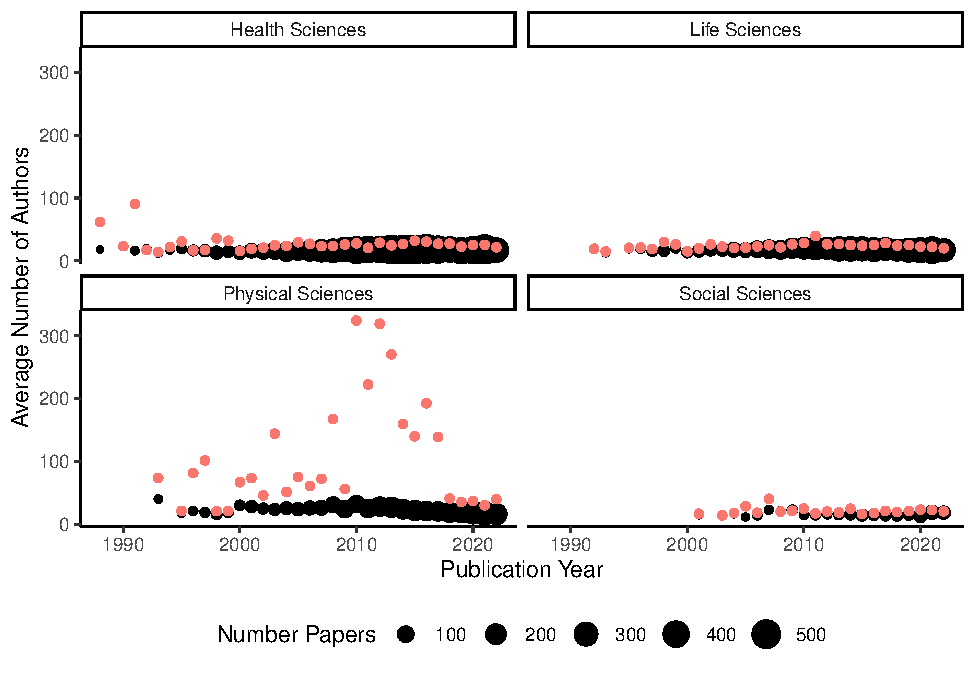
\includegraphics{manuscript_scopus_files/figure-latex/fig-author-year-1.pdf}
\caption{\label{fig:fig-author-year}Number of authors included on big-team science papers per year by subject area. Given the large skew in the data, the left panel presents the median number of authors per manuscript, and the right panel presents the average number of authors per manuscript by year.}
\end{figure}

\textbf{\emph{Career Length}}.

Figure \ref{fig:fig-career} portrays the average career length for
authors involved in BTS publications across years. Career length was
defined as the year of first publication minus the current year, and
higher numbers mean longer careers. To analyze trends over time, we
calculated the average career length for each publication (i.e., average
author career lengths to create one score for each paper) and analyzed a
regression analysis using career length to predict year of publication.
In order to show variance between individuals, we calculated the
standard deviation of career length for each publication and used this
variance as an additional predictor.

Negative career length slopes would indicate more young scholars in
later years (i.e., lower average career length as time increases).
Positive career length slopes would indicate older scholars in later
years (i.e., higher average career length as time increases). Negative
career variance slopes imply that variability decreases over the years,
so the average career length is more homogeneous. Positive career length
slopes imply that variability increases over the years, so the average
career length is varied across individuals (i.e., different stages of
scholars). Figure \ref{fig:fig-heatmap} displays the results for all
regression analyses to compare coefficient strength across and within
each hypothesis.

All values for these analyses were different from zero. The slopes for
the average career length were negative for all four subject areas,
indicating a trend toward younger scientist involvement over time for
each area, with the strongest effect in the Physical Sciences. The
coefficient for variability in career length was also negative for each
of the four subject areas with the highest in the Physical Sciences and
lowest in the Life Sciences. This result indicates a decrease in the
variability of career lengths over time, likely from two sources: 1)
more publications with more authors, thus, lowering variance
estimations, and 2) more young scholars overall. The effect sizes for
this analysis were surprisingly large ranging from \(R^2\) = .25 to .47.
All values and their confidence intervals can be found on our OSF page.

\begin{figure}
\centering
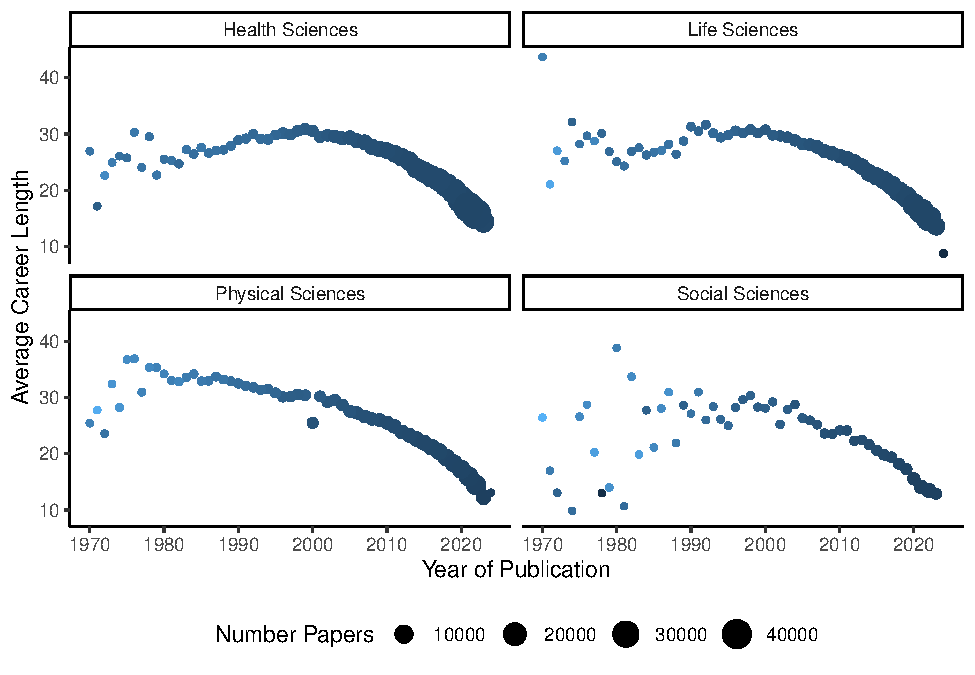
\includegraphics{manuscript_scopus_files/figure-latex/fig-career-1.pdf}
\caption{\label{fig:fig-career}Average career length for big-team science authors. Larger dots indicate more variability in career length for authors by averaging the standard deviation in career length for each manuscript within a year. The data has been filtered to at least 10 publications in a year for this graph.}
\end{figure}

\begin{figure}
\centering
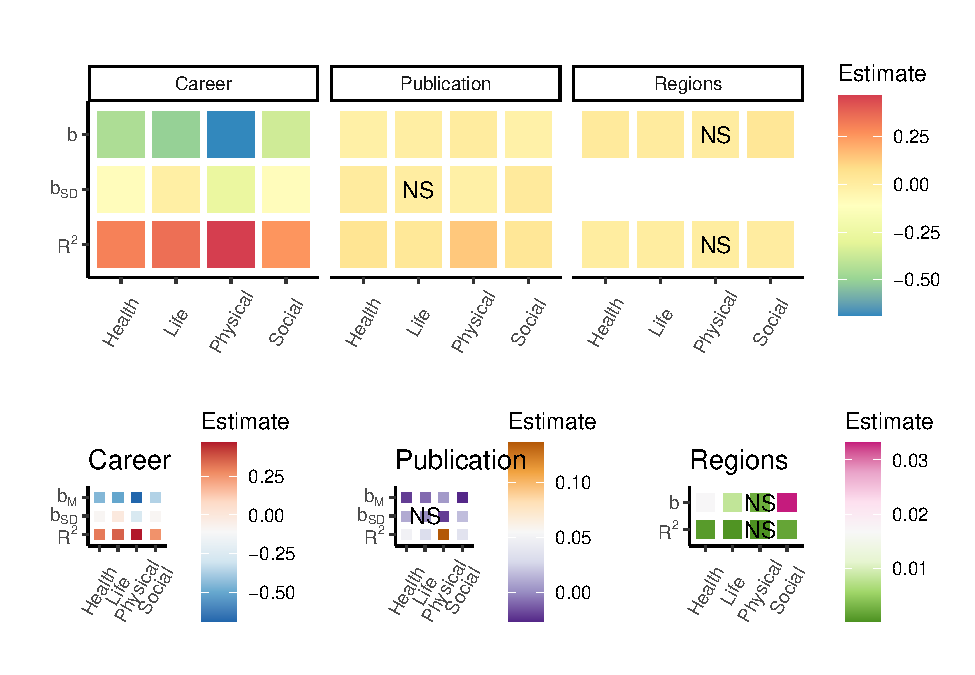
\includegraphics{manuscript_scopus_files/figure-latex/fig-heatmap-1.pdf}
\caption{\label{fig:fig-heatmap}Heatmap results of regression analyses for career length, number of publications, and geopolitical diversity within the region. The top figure represents all results together for comparison across analyses. The bottom row represents individual heatmaps for each hypothesis to distinguish small differences between subject areas for those research questions. Non-significant results are indicated with NS on the plot.}
\end{figure}

\textbf{\emph{Institution}}.

The total number of unique affiliation across all papers was 463876.

\textbf{\emph{Publication Metrics}}.

The average number of publications by authors on big team science papers
is \emph{M} = 38.37 (\emph{SD} = 102.54). The
publication counts were averaged across authors for each publication,
and then these average publication counts were averaged across
publications \emph{M} = 162.50 (\emph{SD} =
155.17). The average variability (i.e., the average
standard deviation with authors of a manuscript) with publication counts
of a paper was \(M_{SD}\) = 164.27 (\(SD_{SD}\) =
127.21).

The same process was completed with \emph{h}-index for each author and
publication. The average \emph{h}-index for authors overall was \emph{M} =
33.65 (\emph{SD} = 127.34, \emph{Med} = 8.00). The
average \emph{h}-index for publications was \emph{M} = 198.87 (\emph{SD}
= 248.78), and the variability of \emph{h}-index across
manuscripts was \(M_{SD}\) = 211.80 (\(SD_{SD}\) =
238.53, \(Med_{Med}\) = 68.00).

We used the same analyses described in the career length section to
analyze trends over time. An increasing slope over time indicates that
individuals who are publishing more are more represented in BTS over
time (i.e., increasing numbers of scholars with higher publication
rates), while a negative slope indicates more researchers with less
publications. A positive slope for the standard deviation of publication
metrics indicates increasing variance over time (i.e., more diversity in
the individual publication rates), while a negative slope would indicate
less diversity in researchers over time. While publication rates do not
represent value as a researcher, they are often used in hiring and
promotion decisions, and we used this variable as a proxy to gauge the
diversity in scholars represented in big teams. As shown in Figure
\ref{fig:fig-heatmap} publication metrics were generally negative for
the average publication metrics, indicating more scholars over time with
lower numbers of publications with the strongest effects in Health and
Social Sciences. The variability of publication counts was not
significant for the Life Sciences but was negative for the Physical
Sciences (less variability over time) and positive for Social and Health
Sciences (more variability and over time). This result indicates that
the Physical Sciences are trending toward scholars with less
publications but also less diverse in number of publications, while the
Health and Social Sciences see more diversity in publication counts and
less published scholars overall.

\textbf{\emph{Geopolitical Regions}}.

\begin{figure}
\centering
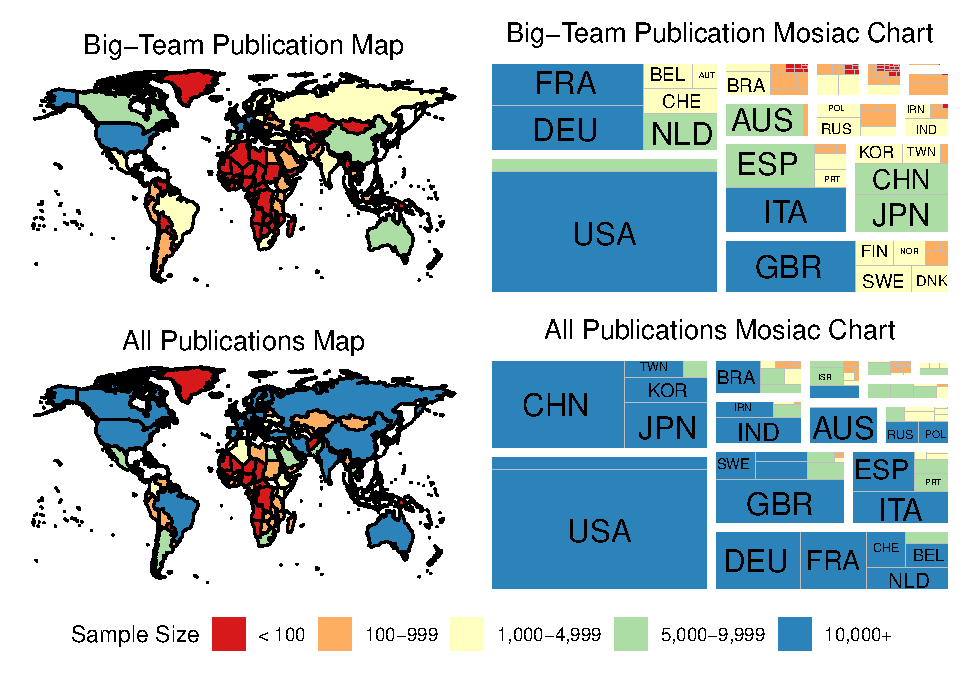
\includegraphics{manuscript_scopus_files/figure-latex/fig-map-both-1.pdf}
\caption{\label{fig:fig-map-both}Geopolitical regions represented in big-team science publications versus all publications. The mosaic plot is grouped by UN subregion with the largest number of publications on the left and smallest on the top right.}
\end{figure}

Author geopolitical region is displayed in Figure
\ref{fig:fig-map-both}. Big team publications appear to be led by North
America and Western Europe, while all publications are led by North
America and East Asia. To understand the change in representation
diversity, we examined if the number of regions in a publication is
predicted by the year of publication. Increasing diversity would be
represented by a positive slope, while decreasing diversity would be
represented by a negative slope. As shown in Figure
\ref{fig:fig-heatmap}, the Physical Sciences do not show a trend of
change in representation, while all other sciences showed a positive
effect increasing in the number of geopolitical regions authors
represent on publications.

Last, we examined the differences in representation for corresponding
author sets versus all other authors. For papers with 10 to 49 authors,
we used the three first authors and the last author to compare against
other authors. For 50 to 99 authors, five first authors plus last were
used, and for all papers with more than 100 authors, we used ten first
authors and the last author as the corresponding author set. We then
calculated the frequencies of each of the UN Sub-Regions for
corresponding authors versus all other authors, converting these values
to proportions. Given the expected small sample sizes of these
contingency tables, we grouped together titles based on the year of
publication. For each grouping, we then calculated the effect size of
the differences in frequencies comparing corresponding authors to all
other authors. Since this data is categorical, we used Cramer's \emph{V} to
represent the effect size. If the effect size includes zero in its
confidence interval (to four decimal places), this result will imply
that first and all other authors represent the same pattern of UN
Sub-Region diversity. Any confidence interval that does include zero
represents a difference in diversity.

\begin{figure}
\centering
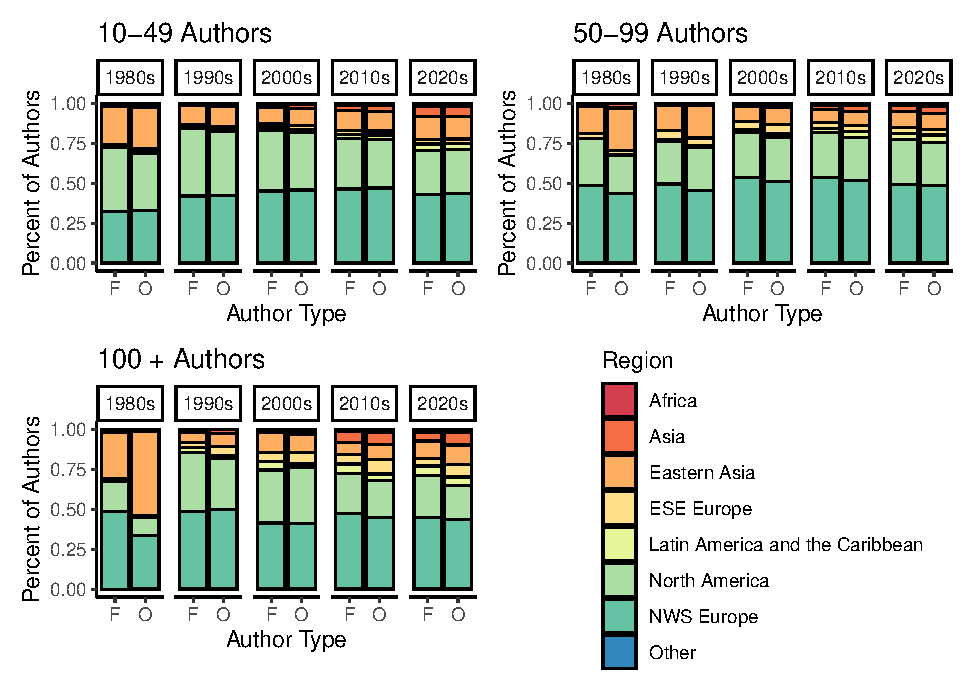
\includegraphics{manuscript_scopus_files/figure-latex/fig-author-gpe-1.pdf}
\caption{\label{fig:fig-author-gpe}A comparison of author affiliation geopolitical regions across decades. F stands for first authors and O stands for other authors.}
\end{figure}

\begin{figure}
\centering
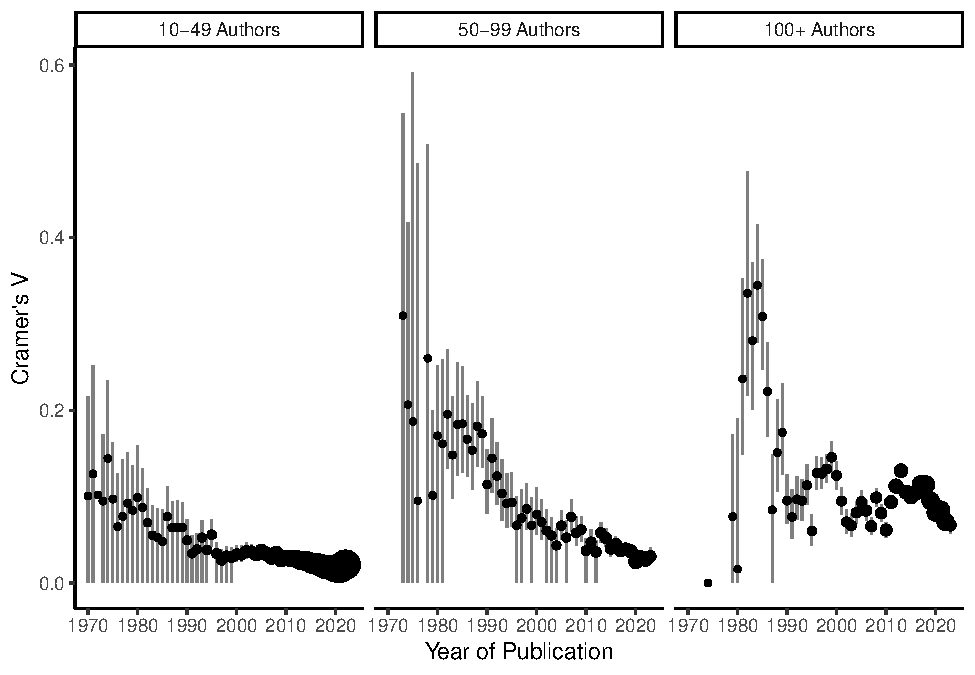
\includegraphics{manuscript_scopus_files/figure-latex/fig-effect-gpe-1.pdf}
\caption{\label{fig:fig-effect-gpe}Effect size of the differences in representation for UN Regions for author affiliations in big-team science papers by year. Larger dots indicate more papers and authors represented in the calculation of effect size.}
\end{figure}

Figure \ref{fig:fig-author-gpe} indicates the percent of authors in
regions. In general, we found the same pattern as the overall analysis
wherein most authors are from Europe and North America. The pattern of
representation is roughly similar for the separation of small, medium,
and large numbers of authors on papers. Across time, the representation
does appear to diversify, with more representation in Asia, Latin
American, and Africa. Figure \ref{fig:fig-effect-gpe} represents the
size of the differences in first/corresponding authors and other authors
across time and number of authors. The differences in representation are
larger for papers with more authors; however, the effects are non-zero
for many of the comparisons. Encouragingly, over time these effects
appear to diminish in size. One limitation with the calculation of
effect sizes for count data is the sensitivity of the data to sample
size (i.e., \(\chi^2\) is upwardly biased by sample size, and \(V\) is
calculated based on this value). While we used the inclusion of zero as
our boundary for ``significance'', the interpretation of the effects is
that most are likely small: \(V\) \textless{} .05:
31.79\%, \(V\) \textless{} .10:
70.20\%, \(V\) \textless{}
.20: 94.04\%.

\hypertarget{discussion}{%
\section{Discussion}\label{discussion}}

In this investigation, we explored the publication rates, areas, and
researchers involved in big team science publications. Over a
half-million articles were published in nearly 15,000 journals since
1970 that qualified as big team science articles (at least ten authors
and ten different affiliations). The areas of publication were aligned
to cancer and genetics research in medicine and oncology for Health and
Life Sciences, physics and chemistry for the Physical Sciences, and
psychology for the Social Sciences All areas of research show an
explosion in growth in the number of publications and the number of
authors included on manuscripts, replicating previous investigations
into this topic area\textsuperscript{50--52}.

Our investigation expands into an exploration of the researchers who
publish in big teams focusing on career length, publication metrics, and
geopolitical affiliation. The number of earlier career scholars is
increasing in publications across the years, indicating that big teams
may be more accessible to different types of individuals, not just
older, more established researchers. This result is especially
interesting given the publish-or-perish model still present in most
institutions, as it may seem that large-scale projects could be a risky
choice for non-permanent researchers. In the authors' experience, big
team projects are often quite slow to publication, incentives may be low
for non corresponding authors if institutions do not value papers
without lead authorship, and there is no guarantee for publication even
with a large group. However, with a large team the distribution of work
could imply less effort on individual non-leading members, and research
has shown that larger-team publications do receive more citations and
appear to have higher impact\textsuperscript{53}.

The results for the number of publications by big team researchers
mimics the findings from career length, with a smaller effect size. In
general, it appears that there is a decrease in the average number of
publications a researcher has when publishing on a big team science
paper over time. This result is likely attributable to the number of
early career scholars joining projects, but also may support increased
accessibility for individuals to be involved in this type of research.
Globalization, the internet, and the focus on interdisciplinary research
are potentially driving forces behind our results, but, hopefully, the
results also point to a decline in scientific gatekeeping\textsuperscript{54,55}.

The variability in the types of researchers involved in publications
also decreased across time in most areas of science with a decrease in
variability for career length. As mentioned, an increase in early career
researchers and numbers of publications could explain this effect
mathematically, potentially with other social influences mentioned
above. The variability in the number of publications is decreasing in
the Physical Sciences, mirroring the career length results, but the
opposite effect was found in the Health and Social Sciences. We see no
clear reason why career variability would decrease while the variability
in the number of publications would increase. The effect sizes for
career length were much larger than the effects for number of
publications. One speculation is the increasing requirements for a
competitive faculty role application. Given the limited number of
positions, one potential way to distinguish their application would be a
larger number of publications in their early career\textsuperscript{56,57}.

The number of geopolitical entities for researcher affiliation is
increasing over time, showing the results of globalization and the
ability to connect across time zones and cultures\textsuperscript{58}. While our
definition of big team science required at least ten different
institutional affiliations, we did not filter papers by geopolitical
region, and thus, a manuscript could rely solely on institutions within
a single country. The Physical Sciences did not show an increase in
diversity of regions represented, however, it could be argued that the
development of large research centers like CERN forced earlier diversity
than other sciences (i.e., because CERN specifically recruited
scientists from sponsoring nations). The Life, Health, and Social
Sciences saw an increase in the number of regions represented with the
highest increase in the Social Sciences. This result likely corresponds
with an increased interest in big team science publications in
psychology\textsuperscript{2,3}, and the desire to diversify the
populations represented in psychological research\textsuperscript{43,44}.

While publications on the whole are diversifying, we did not yet find
equality in the representation for first/corresponding author spots
versus all other authors. In general, first authors appear to be less
diverse, representing more European and North American authors, while
other authors include more Asian and African authors. These effect sizes
were often small, but the inequality still persists across years, even
if they are slowly decreasing. Diverse teams are more likely to have
papers with stronger ``impact''\textsuperscript{59--62} with higher citation metrics for more diverse author lists.
The introduction of contributorship models (e.g., CRediT\textsuperscript{42})
will hopefully continue to push these effects down, as they highlight
each individual's contribution to a manuscript.

The limitations for this research are tied to the availability and
curation of the Scopus dataset. While the number of articles analyzed
for this investigation was large, the criteria for inclusion requires
the correct entry of author affiliations, the correct author linkages
for career length and publication rates, and the correctly marked
geopolitical entity. We had planned to analyze educational levels to
determine if the number of student coauthors (i.e., non-terminal degree)
had increased over time; however, this data was mostly blank within the
Scopus archive. Scopus is a carefully curated dataset, but these
limitations must be kept in mind when interpreting the results.
Publication language diversity was not investigated, and a previous
study indicates that the majority of publications in big databases are
in English\textsuperscript{63}. Certainly, publications in non-English
languages would improve the statistics on diversity in scientific
publishing - but the English language barrier likely exists regardless
of inclusion in databases\textsuperscript{64,65}.

Big teams have the ability to provide high-impact, important research
within scientific publishing, and this report suggests a promising trend
of increasing numbers of publications that include earlier career and
more diverse scholars. These partnerships introduce new challenges to
collaboration from interpersonal conflict, infrastructure, incentives,
to international political situations\textsuperscript{3}. Directed studies
into ways to navigate these situations would be beneficial for policy
makers at institutions, as well as lead teams who organize and complete
these projects. The implications for retention and promotion processes
across a broad span of regions should be explored to improve diversity
with the understanding of the differential impact of incentives for
participating in big team studies.

\newpage

\hypertarget{references}{%
\section{References}\label{references}}

\begingroup
\setlength{\parindent}{-0.5in}
\setlength{\leftskip}{0.5in}

\hypertarget{refs}{}
\begin{CSLReferences}{0}{0}
\leavevmode\vadjust pre{\hypertarget{ref-oed2016}{}}%
\CSLLeftMargin{1. }%
\CSLRightInline{OED. Collaboration. vol. 3 (2016).}

\leavevmode\vadjust pre{\hypertarget{ref-coles2022}{}}%
\CSLLeftMargin{2. }%
\CSLRightInline{Coles, N. A., Hamlin, J. K., Sullivan, L. L., Parker, T. H. \& Altschul, D. \href{https://doi.org/10.1038/d41586-022-00150-2}{Build up big-team science}. \emph{Nature} \textbf{601}, 505--507 (2022).}

\leavevmode\vadjust pre{\hypertarget{ref-forscher2022a}{}}%
\CSLLeftMargin{3. }%
\CSLRightInline{Forscher, P. S. \emph{et al.} \href{https://doi.org/10.1177/17456916221082970}{The Benefits, Barriers, and Risks of Big-Team Science}. \emph{Perspectives on Psychological Science} \textbf{18}, 607623 (2022).}

\leavevmode\vadjust pre{\hypertarget{ref-stewart2017}{}}%
\CSLLeftMargin{4. }%
\CSLRightInline{Stewart, N., Chandler, J. \& Paolacci, G. \href{https://doi.org/10.1016/j.tics.2017.06.007}{Crowdsourcing samples in cognitive science}. \emph{Trends in Cognitive Sciences} \textbf{21}, 736--748 (2017).}

\leavevmode\vadjust pre{\hypertarget{ref-maxwell2015}{}}%
\CSLLeftMargin{5. }%
\CSLRightInline{Maxwell, S. E., Lau, M. Y. \& Howard, G. S. \href{https://doi.org/10.1037/a0039400}{Is psychology suffering from a replication crisis?: What does 'failure to replicate' really mean?} \emph{American Psychologist} \textbf{70}, 487--498 (2015).}

\leavevmode\vadjust pre{\hypertarget{ref-nelson2018}{}}%
\CSLLeftMargin{6. }%
\CSLRightInline{Nelson, L. D., Simmons, J. \& Simonsohn, U. \href{https://doi.org/10.1146/annurev-psych-122216-011836}{Psychology's renaissance}. \emph{Annual Review of Psychology} \textbf{69}, 511--534 (2018).}

\leavevmode\vadjust pre{\hypertarget{ref-zwaan2018}{}}%
\CSLLeftMargin{7. }%
\CSLRightInline{Zwaan, R. A., Etz, A., Lucas, R. E. \& Donnellan, M. B. \href{https://doi.org/10.1017/S0140525X17001972}{Making replication mainstream}. \emph{Behavioral and Brain Sciences} \textbf{41}, e120 (2018).}

\leavevmode\vadjust pre{\hypertarget{ref-auspurg2021}{}}%
\CSLLeftMargin{8. }%
\CSLRightInline{Auspurg, K. \& Brüderl, J. \href{https://doi.org/10.1177/23780231211024421}{Has the Credibility of the Social Sciences Been Credibly Destroyed? Reanalyzing the {``}Many Analysts, One Data Set{''} Project}. \emph{Socius: Sociological Research for a Dynamic World} \textbf{7}, (2021).}

\leavevmode\vadjust pre{\hypertarget{ref-nosek2014method}{}}%
\CSLLeftMargin{9. }%
\CSLRightInline{Nosek, B. A. \& Lakens, D. A method to increase the credibility of published results. \emph{Social Psychology} \textbf{45}, 137141 (2014).}

\leavevmode\vadjust pre{\hypertarget{ref-lebel2018}{}}%
\CSLLeftMargin{10. }%
\CSLRightInline{LeBel, E. P., McCarthy, R. J., Earp, B. D., Elson, M. \& Vanpaemel, W. \href{https://doi.org/10.1177/2515245918787489}{A Unified Framework to Quantify the Credibility of Scientific Findings}. \emph{Advances in Methods and Practices in Psychological Science} \textbf{1}, 389--402 (2018).}

\leavevmode\vadjust pre{\hypertarget{ref-vazire2022}{}}%
\CSLLeftMargin{11. }%
\CSLRightInline{Vazire, S., Schiavone, S. R. \& Bottesini, J. G. \href{https://doi.org/10.1177/09637214211067779}{Credibility Beyond Replicability: Improving the Four Validities in Psychological Science}. \emph{Current Directions in Psychological Science} \textbf{31}, 162--168 (2022).}

\leavevmode\vadjust pre{\hypertarget{ref-maizey2019}{}}%
\CSLLeftMargin{12. }%
\CSLRightInline{Maizey, L. \& Tzavella, L. \href{https://doi.org/10.1016/j.cortex.2018.12.015}{Barriers and solutions for early career researchers in tackling the reproducibility crisis in cognitive neuroscience}. \emph{Cortex} \textbf{113}, 357--359 (2019).}

\leavevmode\vadjust pre{\hypertarget{ref-opensciencecollaboration2015}{}}%
\CSLLeftMargin{13. }%
\CSLRightInline{Open Science Collaboration. \href{https://doi.org/10.1126/science.aac4716}{Estimating the reproducibility of psychological science}. \emph{Science} \textbf{349}, aac4716--aac4716 (2015).}

\leavevmode\vadjust pre{\hypertarget{ref-buttrick2020}{}}%
\CSLLeftMargin{14. }%
\CSLRightInline{Buttrick, N. R. \emph{et al.} \href{https://doi.org/10.1177/2515245920917931}{Many Labs 5: Registered Replication of Vohs and Schooler (2008), Experiment 1}. \emph{Advances in Methods and Practices in Psychological Science} \textbf{3}, 429--438 (2020).}

\leavevmode\vadjust pre{\hypertarget{ref-ebersole2016}{}}%
\CSLLeftMargin{15. }%
\CSLRightInline{Ebersole, C. R. \emph{et al.} \href{https://doi.org/10.1016/j.jesp.2015.10.012}{Many Labs 3: Evaluating participant pool quality across the academic semester via replication}. \emph{Journal of Experimental Social Psychology} \textbf{67}, 68--82 (2016).}

\leavevmode\vadjust pre{\hypertarget{ref-ebersole2020}{}}%
\CSLLeftMargin{16. }%
\CSLRightInline{Ebersole, C. R. \emph{et al.} \href{https://doi.org/10.1177/2515245920958687}{Many Labs 5: Testing Pre-Data-Collection Peer Review as an Intervention to Increase Replicability}. \emph{Advances in Methods and Practices in Psychological Science} \textbf{3}, 309--331 (2020).}

\leavevmode\vadjust pre{\hypertarget{ref-klein2018}{}}%
\CSLLeftMargin{17. }%
\CSLRightInline{Klein, R. A. \emph{et al.} \href{https://doi.org/10.1177/2515245918810225}{Many Labs 2: Investigating Variation in Replicability Across Samples and Settings}. \emph{Advances in Methods and Practices in Psychological Science} \textbf{1}, 443--490 (2018).}

\leavevmode\vadjust pre{\hypertarget{ref-klein2022}{}}%
\CSLLeftMargin{18. }%
\CSLRightInline{Klein, R. A. \emph{et al.} \href{https://doi.org/10.1525/collabra.35271}{Many Labs 4: Failure to Replicate Mortality Salience Effect With and Without Original Author Involvement}. \emph{Collabra: Psychology} \textbf{8}, 35271 (2022).}

\leavevmode\vadjust pre{\hypertarget{ref-mathur2020}{}}%
\CSLLeftMargin{19. }%
\CSLRightInline{Mathur, M. B. \emph{et al.} \href{https://doi.org/10.1177/2515245918785165}{Many Labs 5: Registered Multisite Replication of the Tempting-Fate Effects in Risen and Gilovich (2008)}. \emph{Advances in Methods and Practices in Psychological Science} \textbf{3}, 394--404 (2020).}

\leavevmode\vadjust pre{\hypertarget{ref-skorb2020}{}}%
\CSLLeftMargin{20. }%
\CSLRightInline{Skorb, L. \emph{et al.} \href{https://doi.org/10.1177/2515245920927643}{Many Labs 5: Replication of van Dijk, van Kleef, Steinel, and van Beest (2008)}. \emph{Advances in Methods and Practices in Psychological Science} \textbf{3}, 418--428 (2020).}

\leavevmode\vadjust pre{\hypertarget{ref-bago2022}{}}%
\CSLLeftMargin{21. }%
\CSLRightInline{Bago, B. \emph{et al.} \href{https://doi.org/10.1038/s41562-022-01319-5}{Situational factors shape moral judgements in the trolley dilemma in Eastern, Southern and Western countries in a culturally diverse sample}. \emph{Nature Human Behaviour} \textbf{6}, 880--895 (2022).}

\leavevmode\vadjust pre{\hypertarget{ref-buchanan2023}{}}%
\CSLLeftMargin{22. }%
\CSLRightInline{Buchanan, E. M. \emph{et al.} \href{https://doi.org/10.1038/s41597-022-01811-7}{The psychological science accelerator{'}s COVID-19 rapid-response dataset}. \emph{Scientific Data} \textbf{10}, 87 (2023).}

\leavevmode\vadjust pre{\hypertarget{ref-dorison2022}{}}%
\CSLLeftMargin{23. }%
\CSLRightInline{Dorison, C. A. \emph{et al.} \href{https://doi.org/10.1007/s42761-022-00128-3}{In {COVID}-19 {Health} {Messaging}, {Loss} {Framing} {Increases} {Anxiety} with {Little}-to-{No} {Concomitant} {Benefits}: {Experimental} {Evidence} from 84 {Countries}}. \emph{Affective Science} \textbf{3}, 577--602 (2022).}

\leavevmode\vadjust pre{\hypertarget{ref-jones2021}{}}%
\CSLLeftMargin{24. }%
\CSLRightInline{Jones, B. C. \emph{et al.} \href{https://doi.org/10.1038/s41562-020-01007-2}{To which world regions does the valence{\textendash}dominance model of social perception apply?} \emph{Nature Human Behaviour} \textbf{5}, 159--169 (2021).}

\leavevmode\vadjust pre{\hypertarget{ref-psychologicalscienceacceleratorself-determinationtheorycollaboration2022}{}}%
\CSLLeftMargin{25. }%
\CSLRightInline{Psychological Science Accelerator Self-Determination Theory Collaboration. \href{https://doi.org/10.1073/pnas.2111091119}{A global experiment on motivating social distancing during the COVID-19 pandemic}. \emph{Proceedings of the National Academy of Sciences} \textbf{119}, e2111091119 (2022).}

\leavevmode\vadjust pre{\hypertarget{ref-moshontz2018}{}}%
\CSLLeftMargin{26. }%
\CSLRightInline{Moshontz, H. \emph{et al.} \href{https://doi.org/10.1177/2515245918797607}{The Psychological Science Accelerator: Advancing Psychology Through a Distributed Collaborative Network}. \emph{Advances in Methods and Practices in Psychological Science} \textbf{1}, 501--515 (2018).}

\leavevmode\vadjust pre{\hypertarget{ref-wang2021}{}}%
\CSLLeftMargin{27. }%
\CSLRightInline{Wang, K. \emph{et al.} \href{https://doi.org/10.1038/s41562-021-01173-x}{A multi-country test of brief reappraisal interventions on emotions during the COVID-19 pandemic}. \emph{Nature Human Behaviour} \textbf{5}, 1089--1110 (2021).}

\leavevmode\vadjust pre{\hypertarget{ref-franco2014}{}}%
\CSLLeftMargin{28. }%
\CSLRightInline{Franco, A., Malhotra, N. \& Simonovits, G. \href{https://doi.org/10.1126/science.1255484}{Publication bias in the social sciences: Unlocking the file drawer}. \emph{Science} \textbf{345}, 1502--1505 (2014).}

\leavevmode\vadjust pre{\hypertarget{ref-hubbard1997}{}}%
\CSLLeftMargin{29. }%
\CSLRightInline{Hubbard, R. \& Armstrong, J. S. \href{https://doi.org/10.2466/pr0.1997.80.1.337}{Publication Bias against Null Results}. \emph{Psychological Reports} \textbf{80}, 337--338 (1997).}

\leavevmode\vadjust pre{\hypertarget{ref-nosek2012}{}}%
\CSLLeftMargin{30. }%
\CSLRightInline{Nosek, B. A., Spies, J. R. \& Motyl, M. \href{https://doi.org/10.1177/1745691612459058}{Scientific Utopia: II. Restructuring Incentives and Practices to Promote Truth Over Publishability}. \emph{Perspectives on Psychological Science} \textbf{7}, 615--631 (2012).}

\leavevmode\vadjust pre{\hypertarget{ref-isager2021}{}}%
\CSLLeftMargin{31. }%
\CSLRightInline{Isager, P. M., van 't Veer, A. E. \& Lakens, D. \emph{Replication value as a function of citation impact and sample size}. \url{https://osf.io/knjea} (2021) doi:\href{https://doi.org/10.31222/osf.io/knjea}{10.31222/osf.io/knjea}.}

\leavevmode\vadjust pre{\hypertarget{ref-isager2021a}{}}%
\CSLLeftMargin{32. }%
\CSLRightInline{Isager, P. M. \emph{et al.} \href{https://doi.org/10.1037/met0000438}{Deciding what to replicate: {A} decision model for replication study selection under resource and knowledge constraints.} \emph{Psychological Methods} \textbf{28}, 438--451 (2023).}

\leavevmode\vadjust pre{\hypertarget{ref-10.7554ux2feLife.71601}{}}%
\CSLLeftMargin{33. }%
\CSLRightInline{Errington, T. M. \emph{et al.} \href{https://doi.org/10.7554/eLife.71601}{Investigating the replicability of preclinical cancer biology}. \emph{eLife} \textbf{10}, e71601 (2021).}

\leavevmode\vadjust pre{\hypertarget{ref-silberzahn2018many}{}}%
\CSLLeftMargin{34. }%
\CSLRightInline{Silberzahn, R. \emph{et al.} Many analysts, one data set: Making transparent how variations in analytic choices affect results. \emph{Advances in Methods and Practices in Psychological Science} \textbf{1}, 337356 (2018).}

\leavevmode\vadjust pre{\hypertarget{ref-john2012}{}}%
\CSLLeftMargin{35. }%
\CSLRightInline{John, L. K., Loewenstein, G. \& Prelec, D. \href{https://doi.org/10.1177/0956797611430953}{Measuring the Prevalence of Questionable Research Practices With Incentives for Truth Telling}. \emph{Psychological Science} \textbf{23}, 524--532 (2012).}

\leavevmode\vadjust pre{\hypertarget{ref-grahe2014}{}}%
\CSLLeftMargin{36. }%
\CSLRightInline{Grahe, J. E. \href{https://doi.org/10.1080/00224545.2014.853582}{Announcing open science badges and reaching for the sky}. \emph{The Journal of Social Psychology} \textbf{154}, 1--3 (2014).}

\leavevmode\vadjust pre{\hypertarget{ref-kidwell2016}{}}%
\CSLLeftMargin{37. }%
\CSLRightInline{Kidwell, M. C. \emph{et al.} \href{https://doi.org/10.1371/journal.pbio.1002456}{Badges to Acknowledge Open Practices: A Simple, Low-Cost, Effective Method for Increasing Transparency}. \emph{PLOS Biology} \textbf{14}, e1002456 (2016).}

\leavevmode\vadjust pre{\hypertarget{ref-nosek2015}{}}%
\CSLLeftMargin{38. }%
\CSLRightInline{Nosek, B. A. \emph{et al.} \href{https://doi.org/10.1126/science.aab2374}{Promoting an open research culture}. \emph{Science} \textbf{348}, 1422--1425 (2015).}

\leavevmode\vadjust pre{\hypertarget{ref-mayo-wilson2021}{}}%
\CSLLeftMargin{39. }%
\CSLRightInline{Mayo-Wilson, E. \emph{et al.} \href{https://doi.org/10.1186/s41073-021-00112-8}{Evaluating implementation of the transparency and openness promotion~(TOP) guidelines:~The TRUST process for rating journal policies, procedures, and practices}. \emph{Research Integrity and Peer Review} \textbf{6}, 9 (2021).}

\leavevmode\vadjust pre{\hypertarget{ref-nosek2014}{}}%
\CSLLeftMargin{40. }%
\CSLRightInline{Nosek, B. A. \& Lakens, D. \href{https://doi.org/10.1027/1864-9335/a000192}{Registered Reports: A Method to Increase the Credibility of Published Results}. \emph{Social Psychology} \textbf{45}, 137--141 (2014).}

\leavevmode\vadjust pre{\hypertarget{ref-stewart2020}{}}%
\CSLLeftMargin{41. }%
\CSLRightInline{Stewart, S. \emph{et al.} \emph{Pre-registration and registered reports: A primer from UKRN}. \url{https://osf.io/8v2n7} (2020) doi:\href{https://doi.org/10.31219/osf.io/8v2n7}{10.31219/osf.io/8v2n7}.}

\leavevmode\vadjust pre{\hypertarget{ref-allen2019}{}}%
\CSLLeftMargin{42. }%
\CSLRightInline{Allen, L., O'Connell, A. \& Kiermer, V. \href{https://doi.org/10.1002/leap.1210}{How can we ensure visibility and diversity in research contributions? How the Contributor Role Taxonomy (CRediT) is helping the shift from authorship to contributorship}. \emph{Learned Publishing} \textbf{32}, 71--74 (2019).}

\leavevmode\vadjust pre{\hypertarget{ref-henrich2010}{}}%
\CSLLeftMargin{43. }%
\CSLRightInline{Henrich, J., Heine, S. J. \& Norenzayan, A. \href{https://doi.org/10.1017/S0140525X0999152X}{The weirdest people in the world?} \emph{Behavioral and Brain Sciences} \textbf{33}, 61--83 (2010).}

\leavevmode\vadjust pre{\hypertarget{ref-newson2021}{}}%
\CSLLeftMargin{44. }%
\CSLRightInline{Newson, M., Buhrmester, M., Xygalatas, D. \& Whitehouse, H. \href{https://doi.org/10.1558/jcsr.38413}{Go WILD, not WEIRD}. \emph{Journal for the Cognitive Science of Religion} \textbf{6}, (2021).}

\leavevmode\vadjust pre{\hypertarget{ref-rad2018}{}}%
\CSLLeftMargin{45. }%
\CSLRightInline{Rad, M. S., Martingano, A. J. \& Ginges, J. \href{https://doi.org/10.1073/pnas.1721165115}{Toward a psychology of homo sapiens: Making psychological science more representative of the human population}. \emph{Proceedings of the National Academy of Sciences} \textbf{115}, 11401--11405 (2018).}

\leavevmode\vadjust pre{\hypertarget{ref-aphilos2021}{}}%
\CSLLeftMargin{46. }%
\CSLRightInline{\href{https://doi.org/10.1038/s41567-021-01278-0}{A philosophical case for big physics}. \emph{Nature Physics} \textbf{17}, 661--661 (2021).}

\leavevmode\vadjust pre{\hypertarget{ref-castelnovo2018}{}}%
\CSLLeftMargin{47. }%
\CSLRightInline{Castelnovo, P., Florio, M., Forte, S., Rossi, L. \& Sirtori, E. \href{https://doi.org/10.1016/j.respol.2018.06.018}{The economic impact of technological procurement for large-scale research infrastructures: Evidence from the Large Hadron Collider at CERN}. \emph{Research Policy} \textbf{47}, 1853--1867 (2018).}

\leavevmode\vadjust pre{\hypertarget{ref-collins2003}{}}%
\CSLLeftMargin{48. }%
\CSLRightInline{Collins, F. S., Morgan, M. \& Patrinos, A. \href{https://doi.org/10.1126/science.1084564}{The human genome project: Lessons from large-scale biology}. \emph{Science} \textbf{300}, 286--290 (2003).}

\leavevmode\vadjust pre{\hypertarget{ref-vanbavel2022}{}}%
\CSLLeftMargin{49. }%
\CSLRightInline{Van Bavel, J. J. \emph{et al.} \href{https://doi.org/10.1038/s41467-021-27668-9}{National identity predicts public health support during a global pandemic}. \emph{Nature Communications} \textbf{13}, 517 (2022).}

\leavevmode\vadjust pre{\hypertarget{ref-sinatra2015}{}}%
\CSLLeftMargin{50. }%
\CSLRightInline{Sinatra, R., Deville, P., Szell, M., Wang, D. \& Barabási, A.-L. \href{https://doi.org/10.1038/nphys3494}{A century of physics}. \emph{Nature Physics} \textbf{11}, 791--796 (2015).}

\leavevmode\vadjust pre{\hypertarget{ref-wuchty2007}{}}%
\CSLLeftMargin{51. }%
\CSLRightInline{Wuchty, S., Jones, B. F. \& Uzzi, B. \href{https://doi.org/10.1126/science.1136099}{The increasing dominance of teams in production of knowledge}. \emph{Science} \textbf{316}, 1036--1039 (2007).}

\leavevmode\vadjust pre{\hypertarget{ref-hunter2008}{}}%
\CSLLeftMargin{52. }%
\CSLRightInline{Hunter, L. \& Leahey, E. \href{https://doi.org/10.1007/s12108-008-9042-1}{Collaborative Research in Sociology: Trends and Contributing Factors}. \emph{The American Sociologist} \textbf{39}, 290--306 (2008).}

\leavevmode\vadjust pre{\hypertarget{ref-lariviuxe8re2015}{}}%
\CSLLeftMargin{53. }%
\CSLRightInline{Larivière, V., Gingras, Y., Sugimoto, C. R. \& Tsou, A. \href{https://doi.org/10.1002/asi.23266}{Team size matters: Collaboration and scientific impact since 1900}. \emph{Journal of the Association for Information Science and Technology} \textbf{66}, 1323--1332 (2015).}

\leavevmode\vadjust pre{\hypertarget{ref-lu2007}{}}%
\CSLLeftMargin{54. }%
\CSLRightInline{Lu, Y. \href{https://doi.org/10.1016/j.lisr.2006.10.007}{The human in human information acquisition: Understanding gatekeeping and proposing new directions in scholarship}. \emph{Library \& Information Science Research} \textbf{29}, 103--123 (2007).}

\leavevmode\vadjust pre{\hypertarget{ref-siler2015}{}}%
\CSLLeftMargin{55. }%
\CSLRightInline{Siler, K., Lee, K. \& Bero, L. \href{https://doi.org/10.1073/pnas.1418218112}{Measuring the effectiveness of scientific gatekeeping}. \emph{Proceedings of the National Academy of Sciences} \textbf{112}, 360--365 (2015).}

\leavevmode\vadjust pre{\hypertarget{ref-caplow2017}{}}%
\CSLLeftMargin{56. }%
\CSLRightInline{Caplow, T. \emph{The academic marketplace}. (Routledge, 2017). doi:\href{https://doi.org/10.4324/9781351305969}{10.4324/9781351305969}.}

\leavevmode\vadjust pre{\hypertarget{ref-kyvik2003}{}}%
\CSLLeftMargin{57. }%
\CSLRightInline{Kyvik, S. \href{https://doi.org/10.1023/A:1025475423482}{Changing trends in publishing behaviour among university faculty, 1980-2000}. \emph{Scientometrics} \textbf{58}, 35--48 (2003).}

\leavevmode\vadjust pre{\hypertarget{ref-xie2014}{}}%
\CSLLeftMargin{58. }%
\CSLRightInline{Xie, Y. \href{https://doi.org/10.1126/science.1252743}{{``}Undemocracy{''}: Inequalities in science}. \emph{Science} \textbf{344}, 809--810 (2014).}

\leavevmode\vadjust pre{\hypertarget{ref-freeman2015}{}}%
\CSLLeftMargin{59. }%
\CSLRightInline{Freeman, R. B. \& Huang, W. \href{https://doi.org/10.1086/678973}{Collaborating with People Like Me: Ethnic Coauthorship within the United States}. \emph{Journal of Labor Economics} \textbf{33}, S289--S318 (2015).}

\leavevmode\vadjust pre{\hypertarget{ref-hinnant2012}{}}%
\CSLLeftMargin{60. }%
\CSLRightInline{Hinnant, C. C. \emph{et al.} \href{https://doi.org/10.1016/j.lisr.2012.03.001}{Author-team diversity and the impact of scientific publications: Evidence from physics research at a national science lab}. \emph{Library \& Information Science Research} \textbf{34}, 249--257 (2012).}

\leavevmode\vadjust pre{\hypertarget{ref-jones2008}{}}%
\CSLLeftMargin{61. }%
\CSLRightInline{Jones, B. F., Wuchty, S. \& Uzzi, B. \href{https://doi.org/10.1126/science.1158357}{Multi-university research teams: Shifting impact, geography, and stratification in science}. \emph{Science} \textbf{322}, 1259--1262 (2008).}

\leavevmode\vadjust pre{\hypertarget{ref-yang2022}{}}%
\CSLLeftMargin{62. }%
\CSLRightInline{Yang, Y., Tian, T. Y., Woodruff, T. K., Jones, B. F. \& Uzzi, B. \href{https://doi.org/10.1073/pnas.2200841119}{Gender-diverse teams produce more novel and higher-impact scientific ideas}. \emph{Proceedings of the National Academy of Sciences} \textbf{119}, e2200841119 (2022).}

\leavevmode\vadjust pre{\hypertarget{ref-albarillo2014}{}}%
\CSLLeftMargin{63. }%
\CSLRightInline{Albarillo, F. \href{https://doi.org/10.1080/01639269.2014.904693}{Language in social science databases: English versus non-english articles in JSTOR and scopus}. \emph{Behavioral \& Social Sciences Librarian} \textbf{33}, 77--90 (2014).}

\leavevmode\vadjust pre{\hypertarget{ref-meneghini2007}{}}%
\CSLLeftMargin{64. }%
\CSLRightInline{Meneghini, R. \& Packer, A. L. \href{https://doi.org/10.1038/sj.embor.7400906}{Is there science beyond english?} \emph{EMBO reports} \textbf{8}, 112--116 (2007).}

\leavevmode\vadjust pre{\hypertarget{ref-ramuxedrez-castauxf1eda2020}{}}%
\CSLLeftMargin{65. }%
\CSLRightInline{Ramírez-Castañeda, V. \href{https://doi.org/10.1371/journal.pone.0238372}{Disadvantages in preparing and publishing scientific papers caused by the dominance of the English language in science: The case of Colombian researchers in biological sciences}. \emph{PLOS ONE} \textbf{15}, e0238372 (2020).}

\end{CSLReferences}

\endgroup

\newpage

\hypertarget{appendix-appendix}{%
\appendix}


\hypertarget{supplemental-materials}{%
\section{Supplemental Materials}\label{supplemental-materials}}

\hypertarget{rq1-publisher-information.-1}{%
\subsection{RQ1: Publisher Information.}\label{rq1-publisher-information.-1}}

\textbf{Number of Journals}.

Table \ref{tab:tab-snip} indicates the SNIP values for BTS publications, while Table \ref{tab:tab-snip-all}. The results from these tables indicate that impact values are slightly higher for BTS publications, while the overall median, minimum, and maximum are the same for each grouping.

\begin{table}[tbp]

\begin{center}
\begin{threeparttable}

\caption{\label{tab:tab-snip}Big-Team Science SNIP Values}

\begin{tabular}{llllll}
\toprule
Subject Area & \multicolumn{1}{c}{M} & \multicolumn{1}{c}{SD} & \multicolumn{1}{c}{Minimum} & \multicolumn{1}{c}{Median} & \multicolumn{1}{c}{Maximum}\\
\midrule
Health Sciences & 2.36 & 3.59 & 0.00 & 1.58 & 173.93\\
Physical Sciences & 1.57 & 1.17 & 0.00 & 1.27 & 30.40\\
Social Sciences & 1.94 & 1.72 & 0.00 & 1.52 & 30.40\\
Life Sciences & 2.02 & 1.60 & 0.00 & 1.51 & 19.07\\
\bottomrule
\end{tabular}

\end{threeparttable}
\end{center}

\end{table}

\begin{table}[tbp]

\begin{center}
\begin{threeparttable}

\caption{\label{tab:tab-snip-all}All Journal Articles SNIP Values}

\begin{tabular}{llllll}
\toprule
Subject Area & \multicolumn{1}{c}{M} & \multicolumn{1}{c}{SD} & \multicolumn{1}{c}{Minimum} & \multicolumn{1}{c}{Median} & \multicolumn{1}{c}{Maximum}\\
\midrule
Health Sciences & 1.45 & 2.87 & 0.00 & 1.15 & 173.93\\
Physical Sciences & 1.08 & 0.77 & 0.00 & 0.97 & 30.40\\
Social Sciences & 1.32 & 1.03 & 0.00 & 1.15 & 30.40\\
Life Sciences & 1.19 & 0.86 & 0.00 & 1.06 & 19.07\\
\bottomrule
\end{tabular}

\end{threeparttable}
\end{center}

\end{table}

\hypertarget{rq2-publication-information.-1}{%
\subsection{RQ2: Publication Information.}\label{rq2-publication-information.-1}}

\textbf{Keywords}. Figure \ref{fig:fig-keywords} indicates the most common keywords present for the BTS publications by subject area. The keywords were tokenized into single tokens. Keywords were then lower cased, and all stop words (for example, the, an, of, into, for) were removed. Finally, a frequency count of tokens was tabulated for each subject area, and this count is used to create the final word cloud presented.

\begin{figure}
\centering
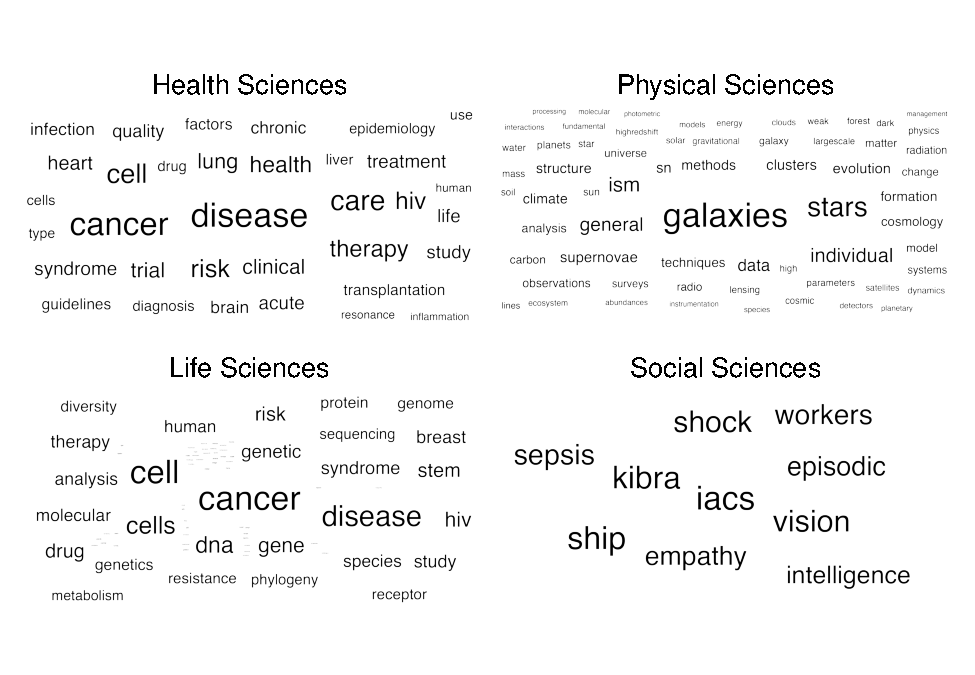
\includegraphics{manuscript_scopus_files/figure-latex/fig-keywords-1.pdf}
\caption{\label{fig:fig-keywords}Keyword Analysis for Each of the Four Subject Areas.}
\end{figure}

\hypertarget{rq3-authors}{%
\subsection{RQ3: Authors}\label{rq3-authors}}

\textbf{Institution}.

Institution was normalized by taking the total number of unique institutions and dividing by the total number of institution listings. The patterns are similar for each decade in that papers are often either half unique institutions or mostly unique institutions overall as shown in Figure \ref{fig:fig-inst}.

\begin{figure}
\centering
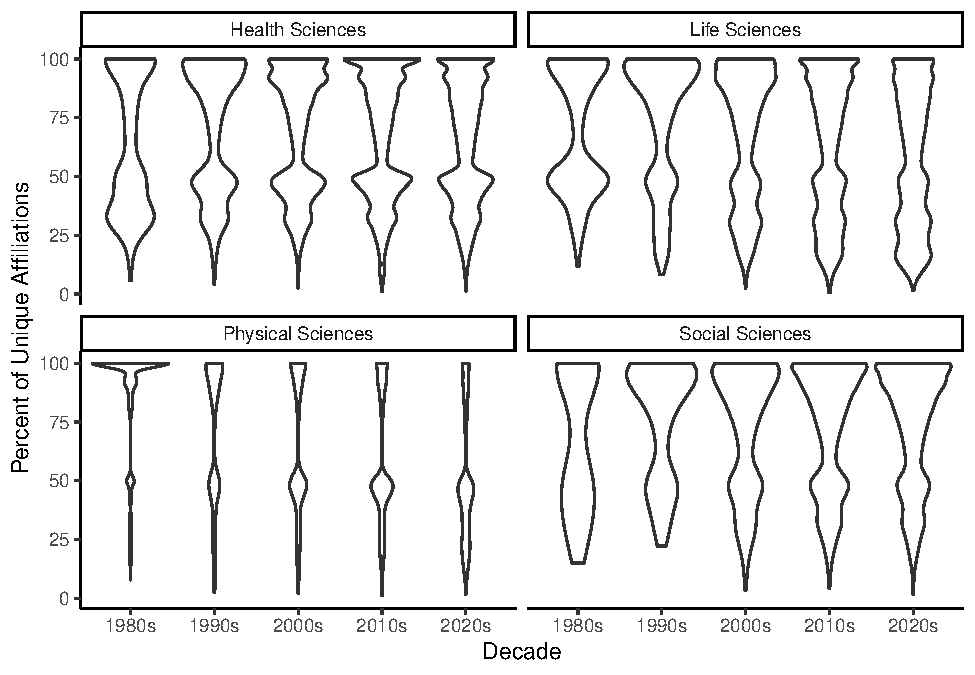
\includegraphics{manuscript_scopus_files/figure-latex/fig-inst-1.pdf}
\caption{\label{fig:fig-inst}Number of unique institutions involved in big-team science papers across decades.}
\end{figure}

\textbf{\emph{Education}}. As noted in our pre-registration, we would only present this variable if we could obtain at least 50\% information on the authors who publish in big team science papers. 95.83\% of the data was not available.

\textbf{\emph{Types of Publications}}.

Types of publications are presented in Figure \ref{fig:fig-pub-types}. The patterns of publications are roughly similar for big team science authors and all authors. It appears that proportionally, big team members are more likely to post preprints in comparison to all authors.

\begin{figure}
\centering
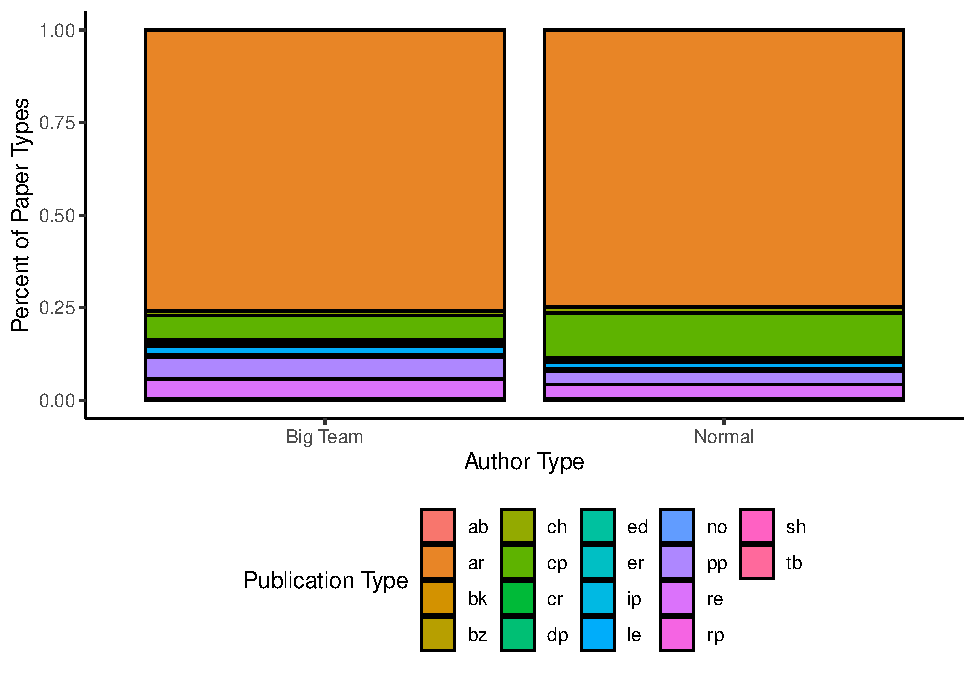
\includegraphics{manuscript_scopus_files/figure-latex/fig-pub-types-1.pdf}
\caption{\label{fig:fig-pub-types}Types of publications for big-team science and all authors.}
\end{figure}


\end{document}
